\documentclass[bibtotoc]{scrreprt}
%\documentclass[bibtotoc,parskip=full]{scrreprt}
\usepackage[utf8]{inputenc}
\usepackage[T1]{fontenc}
\usepackage[english]{babel}
\usepackage{graphicx}
\usepackage{float}	% For placing figures in minipages
\usepackage[hidelinks,linktocpage=true]{hyperref}
\usepackage{xcolor}
\usepackage{lipsum}
\usepackage{tabularx}
\usepackage{longtable}
\usepackage{booktabs}
\usepackage[toc,page]{appendix}
\usepackage{ccicons} % The Creative Commons Icons
\usepackage{perpage} %the perpage package
\MakePerPage{footnote} %the perpage package command

% Add remark without numbering for writing notes

\usepackage{amsthm}
\theoremstyle{remark}
\newtheorem*{remark}{\textcolor{red}{\textbf{Remark}}}

% Add dummy phantomsection for use
\providecommand\phantomsection{}

% Referemces
\usepackage[backend=biber,style=apa]{biblatex}
\addbibresource{bibliography.bib}
\usepackage{csquotes}

% Commands
\newcommand{\needsref}{\textcolor{red}{\textbf{(NEEDS REF)}}}

% glossaries
\usepackage[toc,acronym]{glossaries}
\makeglossary
% Glossary
\newglossaryentry{ps}
{
	name={public sector},
	description={The Public Sector is comprised of organisations that are owned and operated by the government and exist to provide services for its citizens.}
}
\newglossaryentry{artefact}
{
	name={artefact},
	plural={artefacts},
	description={description}
}
\newglossaryentry{agile}
{
	name=agile,
	plural={agility},
	description={The ability to adjust before failure happens}
}
\newglossaryentry{agility}
{
	name={agility},
	description={The state of being agile}
}
\newglossaryentry{antifragile}
{
	name=antifragile,
	plural={antifragility},
	description={The ability to strive for and evolve under stress}
}
\newglossaryentry{antifragility}
{
	name={antifragility},
	description={The state of being antifragile}
}
\newglossaryentry{fragile}
{
	name=fragile,
	plural={fragility},
	description={The quality of being easily broken or destroyed}
}
\newglossaryentry{fragility}
{
	name={fragility},
	description={The state of being fragile}
}
\newglossaryentry{resilient}
{
	name=resilient,
	plural={resiliency},
	description={The ability to recover from failure}
}
\newglossaryentry{resiliency}
{
	name={resiliency},
	description={The state of being resilient}
}
\newglossaryentry{robust}
{
	name=robust,
	plural={robustness},
	description={The ability to resist failure}
}
\newglossaryentry{robustness}
{
	name={robustness},
	description={The state of being robust}
}
\newglossaryentry{volatile}
{
	name=volatile,
	description={Likely to change in a very sudden or extreme way}
}
\newglossaryentry{uncertain}
{
	name=uncertain,
	description={Not known beyond doubt}
}
\newglossaryentry{uncertainty}{
	name={uncertainty},
	description={the state of being uncertain}
}
\newglossaryentry{complex}
{
	name=complex,
	description={A whole made up of complicated or interrelated parts}
}
\newglossaryentry{ambiguous}
{
	name=ambiguous,
	description={Not expressed or understood clearly}
}
\newglossaryentry{stressor}
{
	name={stressor},
	description={An event from outside the system that causes stress}
}
\newglossaryentry{glos_fmea}
{
	name={Failure Mode Effects Analysis},
	description={Is a Six Sigma technique that helps manage quality in a system by investigating how the system will cope with failure}
}
\newglossaryentry{entropy}
{
	name={entropy},
	description={The entropy of the universe increases in all natural processes. Isolated systems tend towards greater disorder and entropy is a measure of that disorder}
}
\newglossaryentry{digitaltransformation}{
	name={digital transformation},
	description={Digital Transformation is the application of digital capabilities to processes, products, and assets to improve efficiency, enhance customer value, manage risk, and uncover new monetisation opportunities.}
}
\newglossaryentry{archframework}{
	name={architecture framework},
	description={An enterprise architecture framework (EA framework) defines how to create and use an enterprise architecture. An architecture framework provides principles and practices for creating and using the architecture description of a system. It structures architects' thinking by dividing the architecture description into domains, layers, or views.}
}
\newglossaryentry{immemorial}{
	name={immemorial},
	description={Reaching beyond the limits of memory, tradition, or recorded history}
}
\newglossaryentry{disintermediation}{
	name={disintermediation},
	description={Disintermediation is the process of cutting out one or more middlemen from a transaction, supply chain, or decision-making process}
}
\newglossaryentry{arduous}{
	name={arduous},
	description={Hard to accomplish or achieve}
}
\newglossaryentry{domain}{
	name={domain},
	plural={domains},
	description={A field of action, thought, influence, etc.: The Domain of Science}
}
\newglossaryentry{convex}{
	name={convex},
	description={Being a continuous function or part of a continuous function with the property that a line joining any two points on its graph lies on or above the graph. In the antifragile theory more upside than downside}
}
\newglossaryentry{concave}{
	name={cavex},
	description={Being a continuous function or part of a continuous function with the property that a line joining any two points on its graph lies below the graph. In the antifragile theory more downside than upside}
}
\newglossaryentry{personalmastery}{
	name={personal Mastery},
	description={Personal mastery is a discipline of continually clarifying and deepening our personal vision, of focusing our energies, of developing patience, and of seeing reality objectively}
}
\newglossaryentry{sharedmentalmodels}{
	name={shared mental models},
	description={Mental models are deeply ingrained assumptions, generalizations, or even pictures of images that influence how we understand the world and how we take action}
}
\newglossaryentry{buildingsharedvision}{
	name={building shared vision},
	description={A practice of unearthing shared pictures of the future that foster genuine commitment and enrollment rather than compliance}
}
\newglossaryentry{teamlearning}{
	name={team learning},
	description={Team learning starts with 'dialogue', the capacity of members of a team to suspend assumptions and enter into genuine 'thinking together'}
}
\newglossaryentry{systemsthinking}{
	name={systems thinking},
	description={The Fifth Discipline of Senge that integrates personal mastery, shared mental models, building shared vision, and team learning}
}
\newglossaryentry{attenuatevariety}{
	name={attenuate variety},
	description={Dampening or reducing the possible outcomes / states. A light that can be turned on and off has the variety of 2. Your hand during Rock, paper, scissors has the variety or 3}
}
\newglossaryentry{amplifyvariety}{
	name={amplify variety},
	description={Amplifying or increasing the possible outcomes / states. A light that can be turned on and off has the variety of 2. Introducing the possibility of setting the light intensity increases the possible states}
}
\newglossaryentry{resourcestoinvest}{
	name={resources to invest},	
	description={Oportonies can only be seized when there are resources free to do see. This can be money but also time and labour. To Survive a black swan investment should be possible}
}
\newglossaryentry{senecabarbell}{
	name={seneca's barbell},	
	description={To be antifragile you need a robust sub-system to which 80\%/90\% predictable value with low risk is situated. The 20\%/10\% should be used for high return on investment activities}
}
\newglossaryentry{insertrandomness}{
	name={insert randomness},	
	description={When insert-low-level stress and fail fails delivers no issues the next step is to insert randomness into the systems. A great example of this is Chaos Engineering by Netflix or the HackerOne bug-bounty system}
}
\newglossaryentry{reducenaiveintervention}{
	name={reduce naive intervention},	
	description={Intervention based on a model and reductionistic logic and ignoring the experience. An example is not listening to the experienced but not so articulate employee, or by ignoring the balance nature has found in a ecosystem}
}
\newglossaryentry{skininthegame}{
	name={skin in the game},	
	description={Make certain that the one making the decision and doing the work has a pain and gain relation with the outcome. This goes beyond having a feedback system in place. This is goed beyond having KPI’s in place. An example is that when working Agile scrum, the product owner should be a co-worker in the team for whom the solution is being build}
}
\newglossaryentry{topdowncc}{
	name={Top-Down Command \& Control},
	description={Top-Down command and control is in an organisation that a employee is not free to decide to go left or right but has to follow orders. The careful design of an iPhone or a good pen is also an example of limited freedom of movement in the product itself}
}
\newglossaryentry{micromanagement}{
	name={micromanagement},
	description={Micro-management is about the freedom in the use of the product. When there are minitious working instructions available in a business process the employee has no freedom in the execution of the job. Another great example is a lego building block. It is engineered and fabricated into the greatest detail creating a building block that is almost completely robust. Lego has a very small resilience behaviour through engineering}
}
\newglossaryentry{redundancy}{
	name={redundancy},
	description={Redundancy is about having not a single point of failure by making use of duplication. An example is a backup electricity generators. Another example is local government as backup system of the central government}
}
\newglossaryentry{modularity}{
	name={modularity},
	description={Modularity is the degree that components may be separated and recombined, often with the benefit of flexibility. For example the finance team and the marketing team. Another example is the user-interface module and the data storage module}
}
\newglossaryentry{loosely coupled}{
	name={loosely coupled},
	description={Loosely coupled is the degree of dependency on the exact working of another module. For example when the color-schema of a website is changed it is preferred that this does not impact the functioning of the website. Another example is that when there are new employees introduced at the finance department the taste of the coffee changes. It is important to understand that there is always some degree of coupling}
}
\newglossaryentry{diversity}{
	name={diversity},
	description={Diversity is internally not being a mono-culture and externally having options. For example having two different coffee suppliers. Or having a diverse team}
}
\newglossaryentry{optionality}{
	name={optionality},
	description={Optionality is an idea advanced by Nassim Taleb in his book Antifragile. At the most basic level, optionality just means having lots of options. If you develop a skill with many possible job opportunities, you have more optionality than someone who develops a skill that only has one or two job opportunities}
}
\newglossaryentry{nonmonotonicity}{
	name={non-monotonicity},
	description={Non-monotonicity is about not only learning from the good but als from the bad. For example the lessons learned during a retrospective session}
}
\newglossaryentry{emergence}{
	name={emergence},
	description={Emergence refers to the existence or formation of collective behaviors, what parts of a system do together that they would not do alone}
}
\newglossaryentry{selforganisation}{
	name={self organisation},
	description={Self-Organisation is a process where some form of overall order arises from local interactions between parts of an initially disordered system. For example students sitting together in the school cafeteria}
}
\newglossaryentry{insertlowlevelstress}{
	name={insert low-level stress},
	description={Continuous Improvement is achieved by inserting low-level of stress continuously into a learning system. This will keep the system sharp all the time}
}
\newglossaryentry{networkconnections}{
	name={network-connections},
	description={A network is created by connections to other nodes. More connections increases potential for optionality for new constructions and also new functionalities}
}
\newglossaryentry{failfast}{
	name={fail fast},
	description={The attributes ''diversity'', ''non-monotonicity'', ''emergence'', ''self-organisation'', ''insert low-level stress'', and ''network-connections'' combined enables the possibility to execute the strategy to embrace the adagium ''Fail Fast''.}
}
\newglossaryentry{foster}{
	name={foster},
	description={To promote the growth or development of}
}
\newglossaryentry{parliamentaryinquiry}{
	name={parliamentary inquiry},
	plural={parliamentary inquiries},
	description={The parliamentary committee of inquiry is a particular type of temporary committee of the House. The parliamentary inquiry is the most powerful instrument the Dutch parliament has at its disposal to carry out its duty to scrutinize the work of the government}
}
\newglossaryentry{houseofthorbecke}{
	name={the House of Thorbecke},
	description={In 1848, as minister, Thorbecke laid the foundations for the current administrative division and task demarcation. In 1850 and 1851 he established the Provinces Act and the Municipalities Act. We therefore also speak of 'the House of Thorbecke'}
}
% Acronyms (abbreviations)

\newacronym{vuca}{VUCA}{Volatility, Uncertainty, Complexity and Ambiguity}
\newacronym{lcm}{LCM}{Least Common Multiple}
\newacronym{cc}{CC}{Creative Commons}
\newacronym{eaal}{EAAL}{Extended Antifragile Attribute List}
\newacronym{cas}{CAS}{Complex Adaptive System}
\newacronym{isv}{ISV}{Independent Software Vendor}
\newacronym{ea}{EA}{Enterprise Architecture}
\newacronym{iot}{IoT}{Internet of Things}
\newacronym{vsm}{VSM}{Viable Systems Model}
\newacronym{asd}{ASD}{\Gls{antifragile} Systems Design}
%\newacronym{fmea}{FMEA}{Failure Mode Effects Analysis}
\newacronym{fmea}{FMEA}{\gls{glos_fmea}}
\newacronym{is}{IS}{Information System}
\newacronym{sos}{SoS}{Systems-of-Systems}

% Document information
\title{Accelerating in a world of chaos}
\subtitle{by using Enterprise Architecture with the concept Antifragility}
\author{J.R. Bliekendaal}

\begin{document}				%	Start the document body

	% Head of thesis

	%\include{contents/coverpage}
	%\chapter*{Executive Summary}
\label{executivesummary}
The Greek philosopher Heraclitus once said that one constant since the beginning of time is change. His central claim is summed up in the phrase Panta Rhei ("life is flux"), recognising life's essential, underlying essence as change. Nothing in life is permanent, nor can it be, because the very nature of existence is change. The Dutch public sector deals with many changes in its environment. Changes follow one another at lightning speed. These are changes such as new technologies, social developments and political priorities. In recent years, the external environment placed new and increasingly compelling demands on the functioning of public organisations. The \gls{ps} finds it challenging to adapt to the expected speed of change. ''There is a need to invest for an even a better government that can respond adequately and flexibly to unforeseen circumstances.'' was plead to 'informateur'\footnote{An '\textit{informateur} is responsible to explore possible governing alliances after elections.}' Schippers \parencite{Secretarissen-generaal2018}. To cope with or even seize opportunities in a dynamic, complex, unpredictable environment, we need to create public organisations that are responsive and adaptive.

This speed of change confronts policy-makers with high demands on their steering skills. The public sector started an improvement program for information provisioning to deal with the increasingly compelling demands on the functioning of public organisations. The improvement program positions Enterprise Architecture as supportive of the proposed improvements, specifically the \acrfull{nora} and the \acrfull{ear}. \gls{ea} is defined as a tool by the Dutch \gls{ps} to support with the implementation of changes.

The Dutch \gls{ps} wants to change toward being more adaptive and responsive. It was proposed by \textcite{Steen2018} to use \gls{antifragile} from \textcite{Taleb2012} to deal with disruptive change.  However, how can the Dutch \gls{ps} achieve \gls{antifragility} with support of \gls{ea}? What are \gls{antifragile} success factors relevant to the Dutch \gls{ps}, and what are \gls{ea} success factors in achieving it? Hence, our research question: \emph{'What are success factors of \gls{ea} and \gls{antifragile} that positively influence the contribution of \gls{ea} in achieving \gls{antifragility} in the Dutch \gls{ps}?'}

We can conclude --- based on our used data sets --- that there are fourteen \glspl{attribute} that are potential success factors. We identified the first seven potential success factors in all three research tools. We identified the last seven in two of three research tools. Alternatively, through literature and confirmed by interviews or through interviews and validated by the expert group. We identified two potential attributes that were not found in literature and can be unique for the Dutch \gls{ps}. In our opinion, these could make the difference for the Dutch \gls{ps} as possible 'key' differentiators. We recommended starting with the first seven, possibly with the two possible 'key' success factors for the Dutch \gls{ps}.
\begin{table}[H]
	\centering
	\small
	\begin{tabular}{@{}cll@{}}
		\toprule
		\textbf{\#} & \textbf{Attribute} & \textbf{Category} \\%
		\midrule
		1 & \Gls{optionality} & \Gls{antifragile} \\%
		2 & \Gls{failfast} & \Gls{antifragile} \\%
		3 & \Gls{resourcestoinvest} & \Gls{antifragile} \\%
		4 & \Gls{systeminenvironment} & \gls{ea} \\%
		5 & \Gls{environmentallearning} & \gls{ea} \\%
		6 & \Gls{intraorganisationalcoherency} & \gls{ea} \\%
		7 & \Gls{systeminenvironmentcoevolutionlearning} & \gls{ea} \\%
		\hdashline %
		8 & \Gls{nonmonotonicity} & \Gls{antifragile}  \\%
		9 & \Gls{selforganisation} & \Gls{antifragile}  \\%
		10 & \Gls{senecabarbell} & \Gls{antifragile}  \\%
		11 & \Gls{safeworkingenvironment}\textsuperscript{*} & \Gls{antifragile}  \\%
		12 & \Gls{holisticsystemicstance} & \gls{ea}  \\%
		13 & \Gls{organisationallearning} & \gls{ea}  \\%
		14 & \Gls{adapttobusinesslanguage}\textsuperscript{*} & \gls{ea}  \\%
		\bottomrule
		\multicolumn{2}{l}{* Not found in literature}
	\end{tabular}%
	\caption*{Potential success factors}
	\label{executive:potentialsuccess}%
\end{table}%
The concept of \gls{antifragile} is relatively young, and as far as we have been able to find, it has not been used in practice in the context of the Dutch \gls{ps}. Little information was therefore available to perform a quantitative analysis. We did choose to use the qualitative research method. The challenge of this method was the validation of results. How could we reduce possible subjectivity? We reduced subjectivity by applying triangulation with multiple research tools.

We performed a literature study. We distilled a list of possible success factors on \gls{antifragile} and \gls{ea}.  We used semi-structured interviews to have the possibility to capture more information than a structured interview. We selected interviewees from the public sector with a role as \gls{cxo} to get the business perspective of the Dutch \gls{ps}. We validated our findings while at the same time we collected new data. The result after analysis was a selection of fourteen possible success factors. Our last validation step was the use of an expert group. We used a different perspective for the expert group members than for the interviewees. We decide to use the \gls{ea} perspective of the Dutch \gls{ps}. We used a group support system for the expert group session for brainstorming and rating possible success factors. After the expert group analysis, the results were a set of fifteen validated possible success factors.

We combined the literature study results, interviews, and expert group. We analysed the possible success factors on the occurrences over the three tools and ranked the possible success factors. We selected the success factors with three and two occurrences as potential success factors. We ranked them based on occurrences.


	\begin{titlepage}
	\begin{center}
		\vspace*{1cm}
		
		\Huge
		\textbf{Accelerating in a world of chaos}
		
		\vspace{0.5cm}
		\large
		
		by using Enterprise Architecture with the concept Antifragility
		
		\vspace{1.5cm}
		\Large
		\textbf{J.R. Bliekendaal}
		
		\vfill
		\large
		A thesis submitted in fulfilment of the requirements\\
		for the degree of Master of Enterprise IT Architecture (MSc)
		
		\vspace{0.8cm}
	
			\includegraphics[width=6cm]{images/ams-logo}
		
		\vspace{0.8cm}
		
		\Large
		Antwerp Management School\\
		Belgium\\
		\today
		
	\end{center}
\end{titlepage}		%	Add the title page
	\thispagestyle{plain}
\pagenumbering{gobble}
\begin{flushright}
''It is quite perplexing that those from whom we have\\
benefited the most aren’t those who have tried to help\\
us (say with ''advice'') but rather those who have\\
actively tried - but eventually failed - to harm us.''\\

\textit{- Nassim Nicholas Taleb}
\end{flushright}

\begin{flushright}
''A consistency proof for [any] system can be carried out\\
only by means of modes of inference that are not\\
formalized in the system itself.''\\

\textit{- Kurt Gödel}
\end{flushright}

\begin{flushright}
''Reality is created by the mind.\\
We can change our reality by changing our mind.''\\

\textit{- Plato}
\end{flushright}

\begin{flushright}
''But he who neither thinks for himself nor\\
learns from others, is a failure as a man.''\\

\textit{- Hesiod}
\end{flushright}

\begin{flushright}
''The only constant is change.''\\

\textit{- Heraclitus}
\end{flushright}			%	Quotes
	\thispagestyle{plain}
\pagenumbering{gobble}
	\begin{tabular}{p{0.3\textwidth}p{0.7\textwidth}}
		\textbf{Thesis Information} & \\
		Title: & Accelerate in a world of chaos by using Enterprise Architecture with the concept antifragile \\
		Language: & British English \\
		Reference Style: & \href{https://apastyle.apa.org/products/publication-manual-7th-edition}{APA Reference Style 7.0}\\
		DOI: & tbd \\
		DOI Reference: & tbd \\
		Copyright & \copyright\ 2022 J.R. Bliekendaal\\
		License: & \href{https://creativecommons.org/licenses/by-sa/4.0/}{\ccbysa\ This work is licensed under a CC-BY-SA 4.0 license.}\\
	\end{tabular}

\vspace{\baselineskip}

	\begin{tabular}{p{0.3\textwidth}p{0.7\textwidth}}
		\textbf{Thesis Project} & \\
		GitHub: & \url{https://github.com/JRBliekendaal/master-thesis/}\\
	\end{tabular}

\vspace{\baselineskip}

	\begin{tabular}{p{0.3\textwidth}p{0.7\textwidth}}
		\textbf{Author} & \\
		Name: & René Bliekendaal, BSc. \\
		ORCID: & \href{https://orcid.org/0000-0002-5449-6449/}{\includegraphics[scale=0.45]{images/ORCIDiD_icon} 0000-0002-5449-6449}\\
		Email: & \href{mailto:jrbliekendaal@gmail.com}{jrbliekendaal@gmail.com}\\
		LinkedIn: & \url{https://www.linkedin.com/in/bliekendaal/}\\
	\end{tabular}

\vspace{\baselineskip}

	\begin{tabular}{p{0.3\textwidth}p{0.7\textwidth}}
		\textbf{Promotor} & \\
		Name: & Prof. Dr. Ing. Hans Mulder \\
		ORCID: & \href{https://orcid.org/0000-0002-3304-9711/}{\includegraphics[scale=0.45]{images/ORCIDiD_icon} 0000-0002-3304-9711}\\
		Email: & \href{mailto:hans.mulder@ams.ac.be}{Hans.Mulder@ams.ac.be}\\
		LinkedIn: & \url{https://www.linkedin.com/in/jbfmulder/}\\
	\end{tabular}

\vspace{\baselineskip}

	\begin{tabular}{p{0.3\textwidth}p{0.7\textwidth}}
		\textbf{Co-Promotor} & \\
		Name: & Edzo A. Botjes, MSc. \\
		ORCID: & \href{https://orcid.org/0000-0003-0097-7375/}{\includegraphics[scale=0.45]{images/ORCIDiD_icon} 0000-0003-0097-7375}\\
		Email: & \href{mailto:e.a.botjes@gmail.com}{e.a.botjes@gmail.com}\\
		LinkedIn: & \url{https://www.linkedin.com/in/edzob/}\\
	\end{tabular}

\vspace{\baselineskip}

	\begin{tabular}{p{0.3\textwidth}p{0.7\textwidth}}
		\textbf{Sponsor} & \\
		Name: & mr. Maarten Hillenaar \\
		LinkedIn:	&	\url{https://www.linkedin.com/in/maarten-hillenaar/}\\
		Company:	&	Centric Public Sector Solutions\\
		Website:	&	\url{https://www.centric.eu}
	\end{tabular}

\vspace{\baselineskip}

	\begin{tabular}{p{1\textwidth}}
		\textbf{Keywords} \\
		agile, agility, resilient, resiliency, robust, robustness, antifragility, antifragile, enterprise architecture, it architecture, architecture governance, architecture principles, enterprise engineering, public sector, independent software vendor, organisational design, delphi method, triangulation\\%
	\end{tabular}
 %	Thesis Information
	\pagenumbering{roman}				%	Set pagenumbering to roman
	\phantomsection
\addcontentsline{toc}{chapter}{Acknowledgements}
\chapter*{Acknowledgements}
\lipsum[1]
\bigskip

\noindent Edzo Botjes\\
Hans Mulder\\
Maarten Hillenaar\\
Dieneke Schouten\\
Barry O'Reilly\\
Krista Bliekendaal\\
%Franc Weerwind\\
%Nathan Ducastel\\
%Theo Peters\\
	%	Add acknowledgements
	\thispagestyle{plain}
\phantomsection
\addcontentsline{toc}{chapter}{Abstract}
\begin{center}
	\Large
	\textbf{Accelerating in a world of chaos}
	
	\vspace{0.4cm}
	\large
	by using Enterprise Architecture with the concept Antifragility
	
	\vspace{0.4cm}
	\textbf{J.R. Bliekendaal}
	
	\vspace{0.9cm}
	\textbf{Abstract}
\end{center}

\lipsum[1] 		%	Add the abstract
	\phantomsection
	% Change title of Table of Contents
	\renewcommand*\contentsname{Table of Contents}
	\addcontentsline{toc}{chapter}{Table of Contents}
	\tableofcontents				%	Add the Table of Contents

	% Body of Thesis

	\clearpage
	\pagenumbering{arabic}			%	Set pagenumbering to arabic
	
	\chapter{Introduction}
\label{ch:introduction}
\setcounter{footnote}{0}
The Greek philosopher Heraclitus once said that one constant since the beginning of time is change. However, the fear of change is also a constant. His central claim is summed up in the phrase Panta Rhei ("life is flux"), recognising life's essential, underlying essence as change \parencite{Seibt2022}. Nothing in life is permanent, nor can it be, because the very nature of existence is change. Since times \gls{immemorial}, humans have liked routine, making us feel in control of our lives. When the feeling of loosing control becomes irrational, the ability to control it can become a phobia \parencite{PsychTimes}. Someone with a phobia for change feels like they have no control over their lives due to constant change. These people tend to live in the past and are unwilling to progress, often leading to depression, seriously impacting their professional and personal lives. If a society or country rejects change, there could be no growth and progress \parencite{Mark2010}. The inability to change, progress, or grow can result in stagnation.

The Dutch \gls{ps} deals with many changes in its environment. Changes follow one another at lightning speed. These are changes such as new technologies, social developments and political priorities \parencite[p.~1]{Nijssen2018}. In the past, these were internal changes such as improving the financial and human resource processes, implementing a new way to organise and control, and the professionalisation of management processes. In recent years, the external environment placed new and increasingly compelling demands on the functioning of public organisations \parencite[p.~13]{Eck2009}. The \gls{ps} finds it challenging to adapt to the expected speed of change \parencites{Linders2013}[p.~2]{Wiebes2014}[pp.~5--6]{Auditdienst2019a}[p.~8]{Meijer2019}[pp.~1--2]{Tangi2020}. E.g. ''The processes, while solid, cannot withstand the current pace of change; the dependence on emergency solutions and manual work is increasing'' \parencite[p.~2]{Wiebes2014}. Trying to follow the expected speed of change often gets stuck on embedded norms, bureaucracy, processes, and structures \parencite[p.~1]{Tangi2020}. 

''There is a need to invest for an even a better government that can respond adequately and flexibly to unforeseen circumstances.'' was plead to Schippers\footnote{\url{https://en.wikipedia.org/wiki/Edith_Schippers}}\footnote{Schippers was at that time the appointed '\textit{informateur}' (Dutch). An '\textit{informateur}' is responsible to explore possible governing alliances after elections.} \parencite{Secretarissen-generaal2018}. A responsive and adaptive government is needed to deal with this \parencite[pp.~79--81]{Steen2018}. We need to create public organisations that can cope with or even seize opportunities in a dynamic difficult, unpredictable environment \parencite[pp.~1--2]{Nijssen2018}. 

\section{Introduction to antifragile}
\label{sec:introantifragility}
There are different principles to deal with uncertainty and disruptive changes \parencite[pp.~79--81]{Steen2018}. \Citeauthor{Steen2018} uses \textcite{Taleb2012} to discuss several manifestations for dealing with disruptive change. The five manifestations of \textcite{Taleb2012} provide a framework for the conversation about adaptive organisations \parencite[pp.~79--81]{Steen2018}. We have \gls{fragility}, \gls{robustness}, \gls{resiliency}, \gls{agility}, and \gls{antifragility}. Organisations that find it difficult or impossible to deal with changes are fragile. That does not mean that these organisations are not successful. They are often very sturdy, solid and successful. However, a fragile organisation will run into problems if the environment requires something from those organisations beyond the limits of the organisations capabilities. A \gls{robust} organisation absorbs and resists stess, while \gls{resilient} orgranisations move along with stress but bounce back to the status quo. \Gls{agile} organisations avoid stress just in time but do not gain, and with \gls{antifragility} an organisation gets better from stress. Agile is not acknowledged by \textcite{Taleb2012} and is in this context only used by \textcite{Steen2018}. \Gls{resiliency} is mentioned but \textcite{Taleb2012} only uses \gls{fragile}, \gls{robust}, and \gls{antifragile} for his \gls{triad} (\cref{fig:antifragilesimple}).
\begin{figure}[H]
	\centering
	\includegraphics[width=0.6\linewidth]{images/antifragilesimple}
	\caption[The antifragile triad]{The antifragile triad}
	\label{fig:antifragilesimple}
\end{figure}
\textcite{Taleb2012} coined \gls{antifragile} as an answer to what he calls a \gls{blackswan}. \Glspl{blackswan} are large-scale unpredictable, and rare events of massive consequences \parencite[p.~6]{Taleb2012}. For extremely rare events the standard tools of probability and prediction, such as the normal distribution, do not apply since they depend on a large population and past sample sizes that are never available for rare events. \Gls{antifragile} means that a system gains more than it loses.

\section{Introduction to Enterprise Architecture}
\label{sec:introea}
Due to the political environment and social environmental factors, the public sector deals continuously with changes and adjustments to objectives and missions \parencite{EARbaten}. This continuous change confronts policymakers with high demands on their steering skills. Instruments such as the '\acrfull{nora}', '\acrfull{ear}', and '\acrfull{gemma}' make it easier for policymakers to deal with this. \acrshort{nora}, \acrshort{ear}, and \acrshort{gemma} are reference architectures. A reference architecture describes general structures \parencite[p.~8]{Greefhorst2008}. It is not specific to one organisation. Many organisations can use a reference architecture because it is abstract. Abstract architectures are the basis for more specific architectures \parencite[p.~11]{Greefhorst2008}. They are an essential tool for reuse at an architectural level. Therefore, organisations should draw as much as possible from these architectures. We deduct that there are multiple levels of architecture. Some kind of architecture hierarchy. Traditionally, reference architectures and \acrlong{ea} in the \gls{ps} correspond to the \acrshort{nora} terms of content \parencite{NORAfamilie}. The \acrshort{nora} itself is a daughter of the \acrfull{eira} (\cref{fig:architectureviewonion}).
\begin{figure}[H]
	\centering
	\includegraphics[width=0.5\linewidth]{images/architectureviewonion}
	\caption[Architecture subsidiaries, based on \parencite{Greefhorst2008}]{Architecture subsidiaries, based on \parencite{Greefhorst2008}}
	\label{fig:architectureviewonion}
\end{figure}
The \gls{ps} is used to working with \acrlong{ea} in which \acrlong{ea} the field is between business administration, information science, and computer science which aims to ensure that an organisation develops in the desired direction \parencite{EAwiki}. The \gls{ps} uses \acrlong{ea} to improve interoperability and efficiently use both intra- and inter-organisational systems \parencite[p.~9]{Giskes2020}.

\section{Research}
\label{sec:research}
The \gls{ps} uses \acrlong{ea} to guide and support the \gls{ps} in dealing with continuous change (\cref{sec:introea}). The public sector wants to change to be more adaptive and responsive (\cref{ch:introduction}). To be more adaptive and responsive, \textcite{Steen2018} proposed to use \gls{antifragile} from \textcite{Taleb2012} (\cref{sec:introantifragility}). However, how can we achieve \gls{antifragility} in the \gls{ps} with \acrlong{ea}? What are the possible success factors of \acrlong{ea} and \gls{antifragile} to change the Dutch \gls{ps} to be more adaptive and responsive by using \acrlong{ea} with \gls{antifragility} in the \gls{ps}? One would expect that it is known how \acrlong{ea} can contribute to changing an organisation into a more \gls{antifragile} organisation. However, we could not find information on the combination of \gls{antifragile} and \acrlong{ea} with or without the \gls{ps}. Most research results deal with \gls{antifragility} in application and information architectures. A small number of sources have investigated \gls{antifragility} in combination with organisations and systems. 

We need more information to determine how the \gls{ps} can become more \gls{antifragile} with \acrlong{ea}. We have to determine the success factors that positively influence becoming \gls{antifragile} with \acrlong{ea} (\cref{fig:conceptualmodel}).
\begin{figure}[H]
	\centering
	\includegraphics[width=0.7\linewidth]{images/conceptualmodel}
	\caption[Conceptual Research Model]{Conceptual Research Model}
	\label{fig:conceptualmodel}
\end{figure}

\subsection{Research question}
\label{sub:introresearchquestion}
Our hypotheses is that in the context of the Dutch \gls{ps} there are success factors of \acrlong{ea} and \gls{antifragile} that have a positive influence on the contribution of \acrlong{ea} in achieving \gls{antifragility} (\cref{fig:conceptualmodel}). Following the conceptual research model, we have the following research question:

\vspace{\baselineskip}
\noindent \emph{''What are success factors that positively influence the contribution of \acrlong{ea} in achieving \gls{antifragility} in the Dutch \gls{ps}?''}
\vspace{\baselineskip}

\noindent The following sub-questions support answering the research question:
\begin{enumerate}
	\item{What is the Dutch \gls{ps}?}
	\item{What is \gls{antifragile}?}
	\item{What are possible success factors for \gls{antifragility}?}
	\item{What is \acrlong{ea}?}
	\item{What are possible success factors of \acrlong{ea}?}
	\item{Which possible success factors are relevant for the Dutch \gls{ps}?}
\end{enumerate}
\subsection{Research relevance}
\label{sub:researchrelevance}
\acrshort{ea} has contributed to organisations in being more \gls{robust}, and \gls{resilient}. Using \acrshort{ea} in pursuing \gls{antifragility} will add value to companies by accelerating and growing when there is a \gls{stressor} or a \gls{blackswan}. For some examples of \glspl{stressor} which are relevant to the \gls{ps} see \cref{fig:publicstressors}. The \gls{antifragile} theory is young. \citeauthor{Taleb2012} published the theory in his book ''\Gls{antifragile}: Things that gain from disorder.'' in \citeyear{Taleb2012}. Studies conducted on \acrshort{ea} with the concept of \gls{antifragile} are almost non-existence. The conducted studies are primarily about making IT Systems \gls{antifragile}. \textcites{Botjes2020}{Kastner2017} are exceptions and have researched how to apply \gls{antifragile} in an organisational context. Nevertheless, both concluded that there is more research needed. The former used the lens of Enterprise Engineering, which is closely related to \acrshort{ea}, together with complex adaptive system resilience, while the latter used mostly resilience as its lens. There is still no answer to how \acrshort{ea} can contribute to achieving \gls{antifragility}. Giving more insights on this subject will contribute to the \acrshort{bok} of \acrshort{ea} and \gls{complexityscience} and help others get closer to \gls{antifragility} by using \acrshort{ea}.
{\let\thefootnote\relax\footnote{{\url{https://www.istockphoto.com/en/vector/506120634-84046799}}}}
\begin{figure}[H]
	\centering
	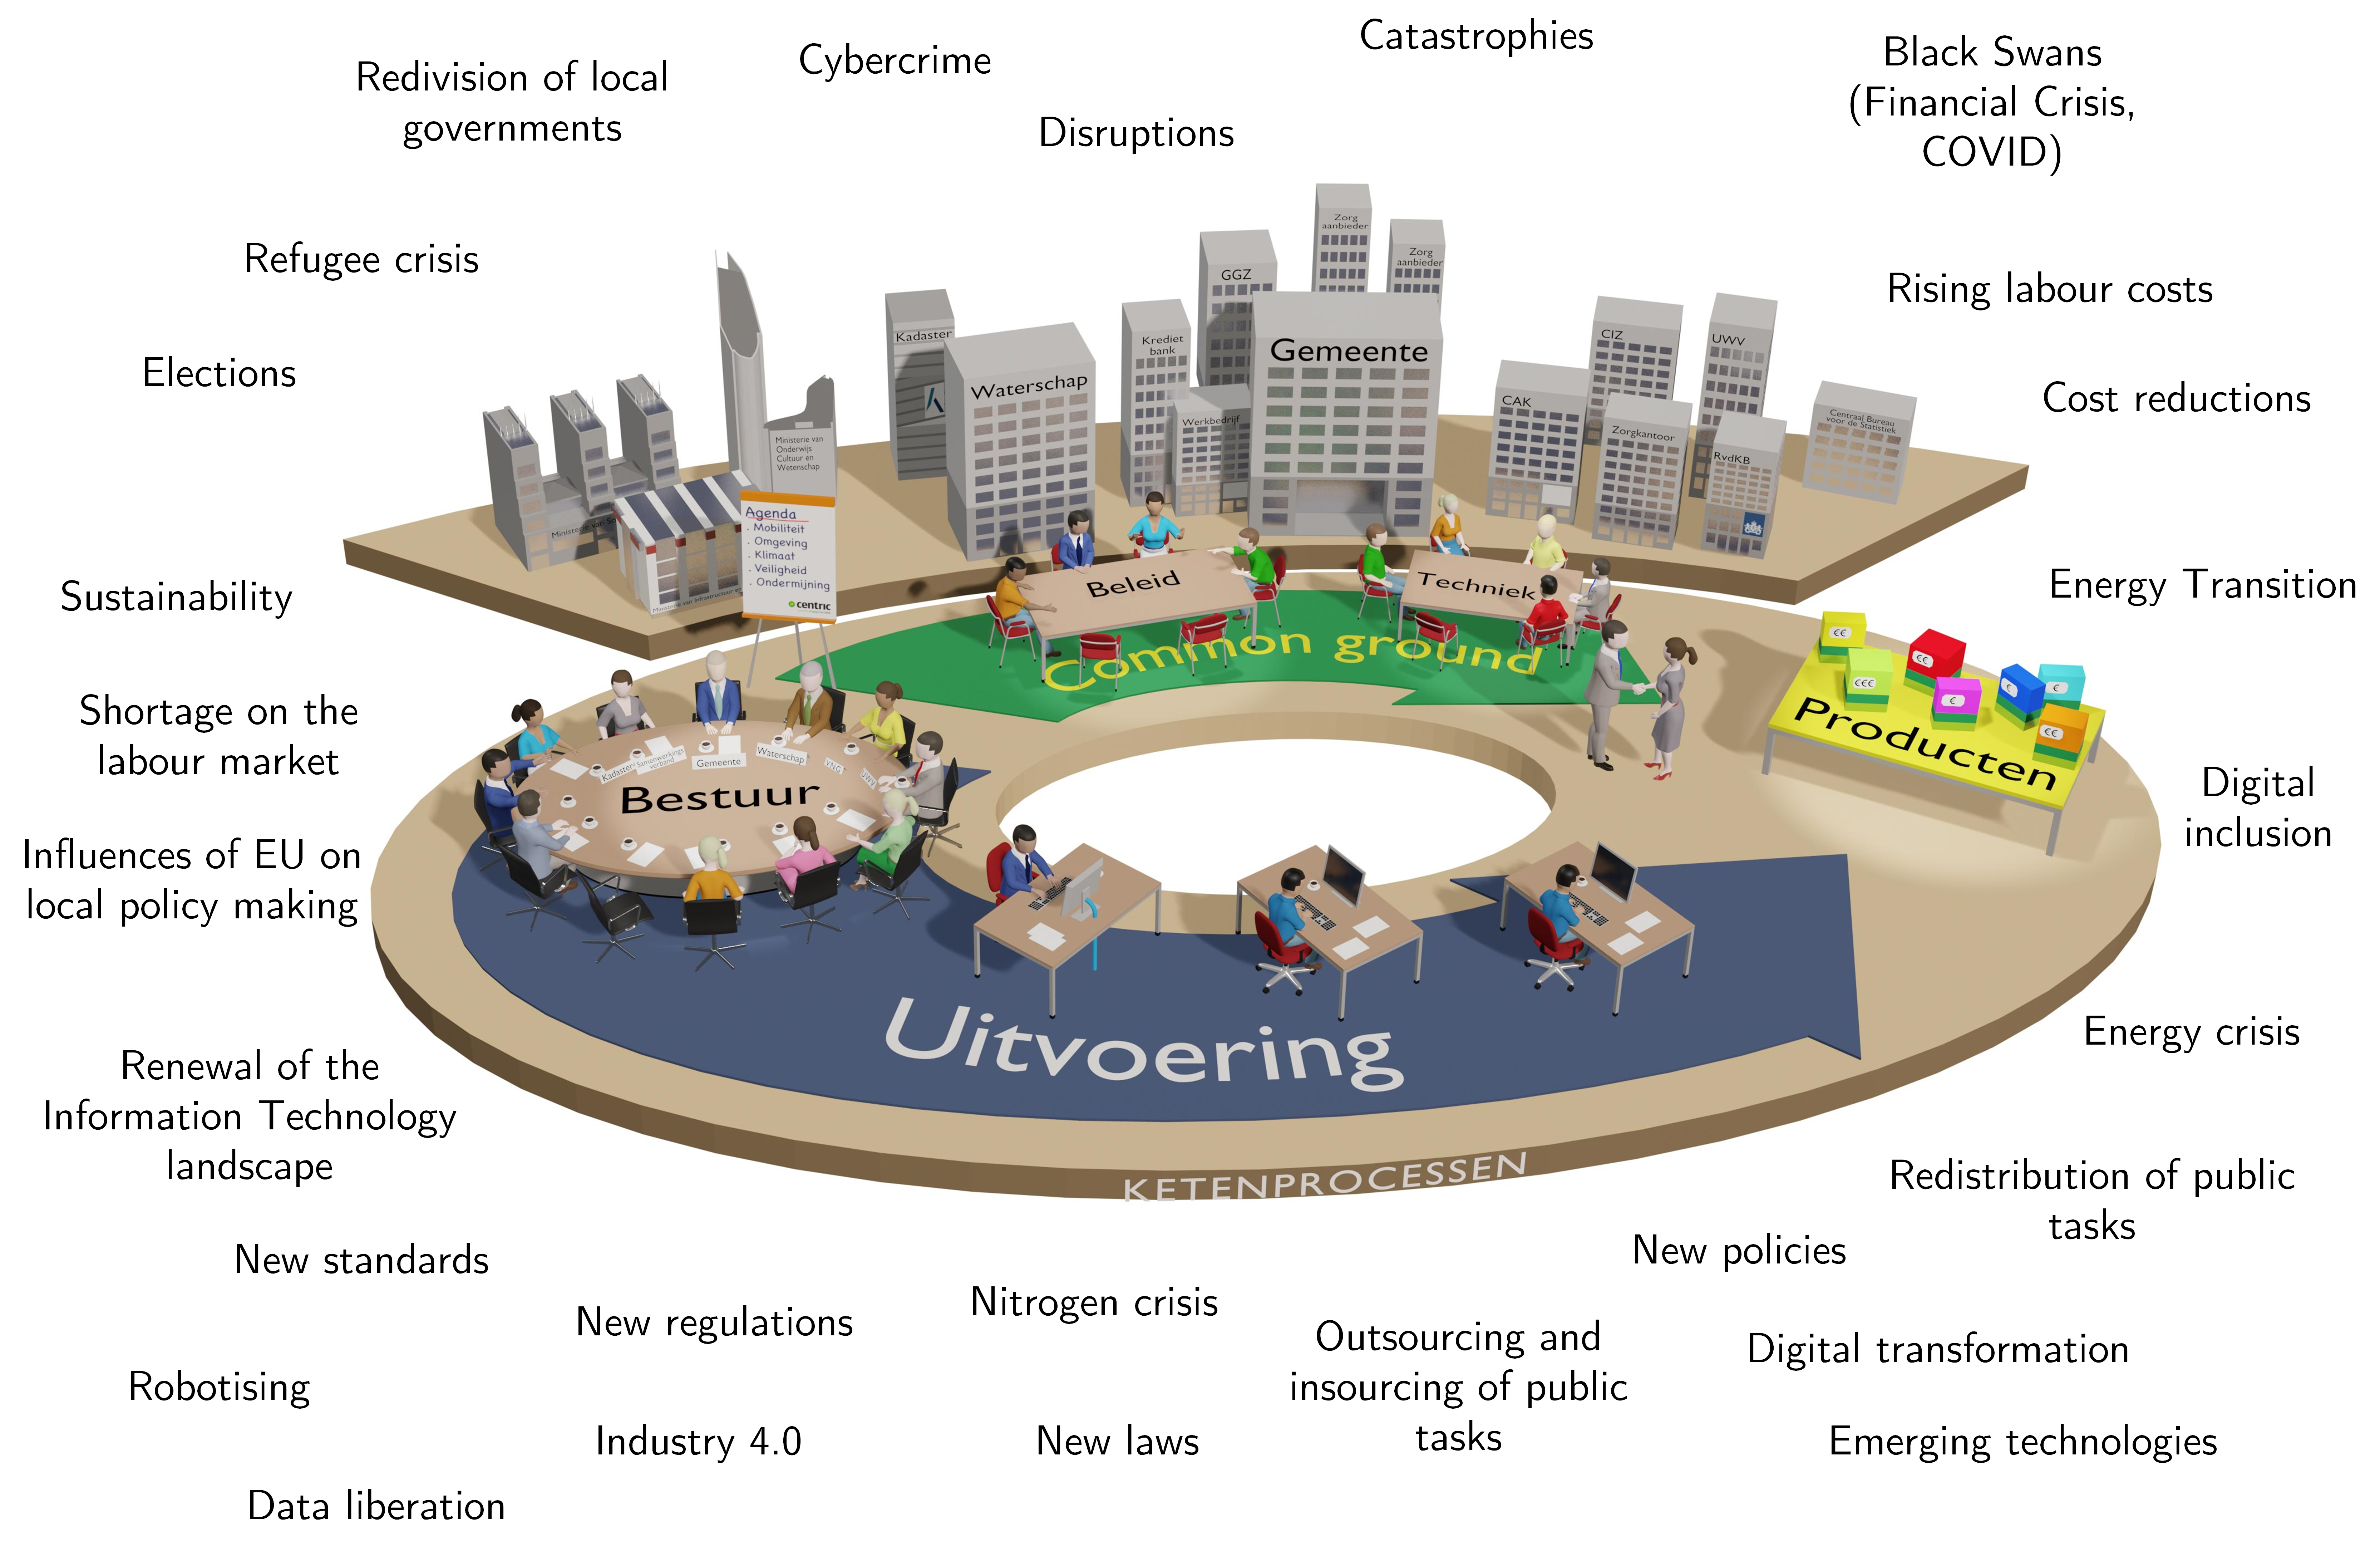
\includegraphics[width=0.8\linewidth]{images/publicstressors}
	\caption[Examples of stressors on the public sector]{Examples of stressors on the public sector}
	\label{fig:publicstressors}
\end{figure}
Because of the \gls{digitaltransformation}, the pace of change is increasing rapidly. In a study by \textcite{Eggers2015}, 96\% of respondents said digital technologies are significantly disrupting the \gls{ps}. According to \textcite{Nurmi2021}, organisations in the public and private sectors alike face the need to manage themselves in an ever more interconnected and fast-paced world. \textcite{Guggenberger2020} states that a paradigmatic change from a mechanistic toward a systemic worldview is ongoing, emphasizing the interconnectedness of participating organizations. 

\begin{remark}
	''The processes, while solid, cannot withstand the current pace of change; the dependence on emergency solutions and manual work is increasing'' \parencite[p.~2]{Wiebes2014}.
\end{remark}

The \gls{digitaltransformation} is not the only \gls{stressor} on the \gls{ps}. There are a lot of internal and external \glspl{stressor}. By being more \gls{robust} or \gls{resilient}, you can only withstand the change or the \gls{stressor}, but you do not gain from it. Governmental organisations and agencies in the Dutch \gls{ps} are searching for methods of dealing with this increased pace and the stressors. There are a lot of indications of this in the discussions and sessions held at \textcite{iBestuurterugblik2021}. The relevance of this research is not only about adding to the \acrshort{bok} of \acrshort{ea} and \gls{complexityscience} but also, in the context of public responsibility, to share the outcome with the \gls{ps} for further study and use.

\section{Design of the thesis}
\label{sec:structure}
The structure of this thesis follows a pattern of divergence before convergence (\cref{fig:design}). We introduce the research (\cref{ch:introduction}). We present the context, explain the design of the thesis, and the necessity of the research. Following, we introduce the main concepts of the research together with a problem statement and research questions. We give a background on the concepts of the research (\cref{ch:theoreticalbackground}). This part also contains the outcome of the literature research we performed based on the approach described in the methodology (\cref{ch:methodology}). The methodology explains the research design, the methods, the quality and the approach. All of these are part of the divergence of the research. We collected much data, but we still have to validate the data and narrow it down to formulate an answer to our research question. The second part of the thesis design will converge the findings.
\begin{figure}[H]
	\centering
	\includegraphics[width=0.9\linewidth]{images/structure}
	\caption[Design of the thesis]{Structure of the thesis}
	\label{fig:design}
\end{figure}
We validate findings with interviews (\cref{ch:interviews}) and an expert group (\cref{ch:expertgroup}). Converging ends with  conclusion and discussions (\cref{ch:conclusionanddiscussions}). The final part of the thesis design is a retrospective of the researcher, the research, and its process (\cref{ch:retrospective}). We have a glossary of terms available at the tail of the thesis to support the reader with used definitions.
 %	Add the introduction
	\chapter{Theoretical background}
\label{ch:theoreticalbackground}

\section{What is a system?}
\label{sec:tbsystem}

\section{Organisation}
\label{sec:tborganisation}

\subsection{Independent Software Vendor}
\label{sub:tbisv}
\lipsum[1]

\section{antifragile}
\label{sec:tbantifragile}
\lipsum[1]

\begin{itemize}
	\item{Randomness}
	\item{Variability}
	\item{Hormesis / Mithridatisation (by taleb) / Antidotum Mithridatium}
\end{itemize}

\subsection{Relation of Antifragile with Robust, Resilient, and Agility}
\label{sub:tbrelatedtoantifragile}
\lipsum[1]

\section{VUCA}
\label{sec:tbvuca}
\lipsum[1]

\section{Enterprise Architecture}
\label{sec:tbea}
\lipsum[1]

\section{Public Sector market}
\label{sec:tbpsmarket}
\lipsum[1]

\section{What is a stressor?}
\label{sec:stressor}
\lipsum[1]


 	%	Add the Theoretical Background
	\chapter{Research Methodology}
\label{ch:research-methodology}

\section{Research Model}
\label{sec:research-model}
	\begin{figure}[h]
		\centering
		\includegraphics[width=12cm]{images/research-model.png}
		\caption[Research Model]{Research Model}
		\label{fig:research-model}
	\end{figure}

\section{Delphi Group}
For the Delphi Group participants see appendix~\ref{app:delphigroupparticipants} \\%

What about the sample size? Normally Delphi is about 100+. What about this research. How large should the sample size be for a qualitative result?

\section{Quality of the Research (old example text)}
\label{sec:quality-of-the-research}
The research was qualitative. The information is based on qualitative information gathered by the researcher
from employees of the organisation. However, with the research approach and transparency, the research can
be validated, can be repeated, so it is reliable and reducible. With the use of managerial models and methods
like Lean, Value Stream Mapping with supporting tools like NEN-ISO/IEC 25011 and ServQual got a nonbiased
result.\\
\begin{itemize}
	\item{\textbf{The validity} of the research is dependent on the right use of the right models and the right methods. The researcher conducted research on which models, frameworks and tools to use. The results and the rationales around the choice of theories, models, frameworks and tools are stated in chapter 4. The sources used for determining the theories, models, frameworks and tools are from scientific and expert sources.}
	\item{\textbf{The reliability} is about the influence of possible errors. For the research, the researcher used methods like triangulation, and sources from scientific reports and expert literature. The number of interviews was too small for the right statistical outcome. To enlarge the reliability of the interviews, the researcher used the same framework of themes for his semi-structured interviews. The transcriptions are placed in the appendixes for transparency. The information gathered with the interviewees is compared with the other interviewees.}
	\item{\textbf{The repeatability} is about getting the same results when the research is conducted again. The researcher uses his research design and research approach, as stated. All the steps taken are put into the research design. If this research design is followed, the same results should follow.}
	\item{\textbf{The reducibility} is about the outcome of the research can be deducted step by step. By using the research model, and the structure of the thesis, every step is reducible.}
\end{itemize}

\begin{itemize}
	\item{Think about Replication}
	\item{Recker types}
	\item{OpenScience}
	\item{Howto falsify?}
	\item{Rigourness}
\end{itemize}


\section{Used research tooling}

\LaTeX\ with the KOMA-Script Report template\\
TeXstudio\footnote{https://www.texstudio.org/}\\
TeX Live\footnote{https://tug.org/texlive/}\\
Dropbox\footnote{https://www.dropbox.com/}\\
GitHub\footnote{https://github.com/} (2 repositories) \\
	Master Thesis Repository\footnote{https://github.com/JRBliekendaal/master-thesis}\\
	Master Thesis Administration Repository\footnote{https://github.com/JRBliekendaal/master-thesis-administration}\\
GitHub Desktop\footnote{https://desktop.github.com/}\\
JabRef\footnote{https://www.jabref.org/} as a reference manager including integration with web browsers\\
PaperPanda\footnote{https://paperpanda.app/} for finding hard to find resources\\
Grammarly\footnote{https://www.grammarly.com/}

Microsoft Excel\\
Microsoft Powerpoint\\
Microsoft Visio\\
Sparx Enterprise Architect\\


Researchgate\\
Web of Science\\
Google Scholar\\
Meetingwizard\footnote{https://www.meetingwizard.nl/}\\


Hardware\\
Dell Windows PC with Windows 10\\
Amazon Kindle Oasis\\

leuchtturm1917 notebooks\\
	%	Add the methodology

	\include{contents/afpublicsector}	% Chapter about the importance in the public sector market
	\include{contents/analysis}		%	Add Analysis Chapter
	\include{contents/artefact}		%	Artefact
	\include{contents/validation}	%	Validation of the artefact by using Delphi

	\chapter{Conclusion and discussions}
\label{ch:conclusionanddiscussions}

\lipsum[1]




\section{Conclusion}
\label{sec:conclusion}

\lipsum[1]

\section{Discussions}
\label{sec:discussions}

\begin{itemize}
	\item{Discuss the definition of System Thinking vs Emergence}
	\item{Discuss Blaming Culture Public Sector}
	\item{Discuss Speaking the language of the Business with EA}
\end{itemize}

\section{Recommendations}
\label{sec:reccomandations}

\lipsum[1]
	%	Add the conclusion
	\chapter{Discussion}
\label{ch:discussion}


\section{Discussion on research}
\label{sec:discussiononresearch}


\subsection{Public Sector}
\label{sub:discussionpublicsector}
Is the public sector in The Netherlands the same as in the rest of the world? This needs further research and needs to be confirmed so that the outcome of this research is universally applicable.

\subsection{Is the Public Sector different then the private sector?}
\label{sub:discussionpublicvsprivate}
\lipsum[1]


\section{Discussion on research quality}
\label{sec:discusssionresearchquality}
\subsection{Size of Delphi Group}
\label{sub:discussionsizeofdelphi}
Is the size of the delphi group large enough to determine....	%	Add the discussion


	\chapter{Blocks of text that can be used}

\section{Validation through an artefact}
Because there is not much known on the applicability of antifragile on Enterprise Architecture, the success factors need to be validated to be true. To validate, the researcher will create an artefact. The Delphi Research Method is used to validate the artefact. By validating the artefact, the researcher can ensure that the success factors are valid with some degree of certainty.\\

\section{CAS System Theory/Complexity sciences}
Quote from AMS011:\\
''The whole is different from the sum of its parts and their interactions'' [61] (p.77) Though emergence, the whole cannog be reduced to the original parts, the whole is considered a new entity or unit. The whole is ''qualitativly different from their parts ... The cannot be meaningfully compared-they are different'' [61] (system holism)

\section{Relevant Laws}
\begin{itemize}
	\item{Second Law of Thermodynamics}
	\item{Conways Law}
	\item{Metcalfe's Law}
\end{itemize}	%	Pieces of text that can be used
	
	\chapter{Chapter Template}
\label{ch:chapter template}
\lipsum[1]

\section{section title}
\label{sec:introtitle}
\lipsum[1]
\subsection{subsection title}
\label{subsec:introtitle}
\lipsum[1]
\subsubsection{subsubsection title}
\label{subsubsec:introtitle}
\lipsum[1]
\paragraph{paragraph title}
\label{par:introtitle}
\lipsum[1]
\section{Building Blocks}
\subsection{table}
\begin{table}[!h]
	\begin{center}
		\begin{tabular}{@{}ccccc@{}}
			\toprule
			What & When & Who & Why & How \\ \midrule
			X    & 1    & 1   & 2   & 3   \\
			Y    & 2    & 45  & 7   & 9   \\
			Z    & 0    & 0   & 1   & 7   \\ \bottomrule
		\end{tabular}
		\caption{Introduction Table}
		\label{tab:introduction}
	\end{center}
\end{table}
\subsection{Picture}
\begin{figure}[!h]
	\centering
	\includegraphics[width=6cm]{images/placeholder-image}
	\caption[Placeholder]{Placeholder}
	\label{fig:placeholder-image}
\end{figure}


\subsection{Glossary}

\begin{verbatim*}
	\gls{antifragile} is not that \gls{fragile}\\
	\Gls{antifragile} is not that \Gls{fragile}\\
	\gls{fragile} is not that \gls{antifragile}\\
	\Gls{fragile} is not that \Gls{antifragile}\\
\end{verbatim*}

Gives:\\
\gls{antifragile} is not that \gls{fragile}\\
\Gls{antifragile} is not that \Gls{fragile}\\
\gls{fragile} is not that \gls{antifragile}\\
\Gls{fragile} is not that \Gls{antifragile}\\

\subsection{Abbreviation}

\begin{verbatim*}
\acrfull{vuca}\\
\acrlong{vuca}\\
\acrshort{vuca}\\
\end{verbatim*}

Gives:\\
\acrfull{vuca}\\
\acrlong{vuca}\\
\acrshort{vuca}\\

\subsection{Citing}
\begin{verbatim*}
	\parencite{Bliek2017}
	\parencite[p. 20]{Bliek2017}
	\citeyear{Bliek2017}
	\citeauthor{Bliek2017}
	\parencite*{Bliek2017}
	\textcite{Bliek2017}
	\parencite{Doe2100,Bliek2017}
\end{verbatim*}
Gives:\\
\parencite{Bliek2017}\\
\parencite[p. 20]{Bliek2017}\\
\citeyear{Bliek2017}\\
\citeauthor{Bliek2017}\\
\parencite*{Bliek2017}\\
\textcite{Bliek2017}\\
\parencite{Doe2100,Bliek2017}	%	Add the Chapter Template

	% Tail of Thesis

	\printbibliography				%	Add Bibliography

	\addcontentsline{toc}{chapter}{List of Figures}
	\listoffigures					%	Add the List of Figures
	\addcontentsline{toc}{chapter}{List of Tables}
	\listoftables					%	Add the list of Tables
	\printglossary[title=Glossary of Terms]
	\printglossary[type=\acronymtype,title=Abbreviations]
	
	\begin{appendices}
		\chapter{Personal Motivation}
I always want to know how something works and why it works the way it works. This eagerness started at a very early age. I always demolished birthday presents into their parts. I wondered how things worked, and I did not stop with the research on the how and why until I understood it. The search for the how and why is a central theme in my life. And because of this, I never stopped learning. When the why is not known, I never give up researching—not knowing the why has only the meaning that nobody has found the answer yet. 

My essential attitude is that of a mathematician or a scientist. I am very binary and sceptical when something is somewhere in between, and I am not fond of shades of grey. So clear definitions is what I pursue. Everything needs an explanation. When I cannot explain, I do not fall back to religion, infinity, approximately, or even ''it is just what it is''. I only accept that we did not find the answer yet.

This journey started with simple things like a toy car or a doll that had a mechanism of saying things. I still think of my little sister, who found hers back in tiny pieces. Later the subjects of research began to be different. Secondary education drove me to understand chemistry, physics, and biology, and I needed an explanation on the who and why to understand it. This drive was probably the main reason I was not perfect in languages. You cannot put consistent rules on languages.  Languages do not have a clear rationale for the rules, and I often heard it is just the way it is.

Grammar school taught me that I was a natural in research, and I decided to pursue research. Firstly at several Universities, but I failed big time. The Universities at that time gave me a lot of answers that it is the way it is, and most of the lecturers did not appreciate me challenging them on the why. Because of this, I started pursuing a job that could fulfil my eagerness for researching, and I found that with an IT Company in the Netherlands.

The technical (hard) side of IT was, at that time, a match made in heaven. Most of the time, it is just like math, you have a clear answer, and you know why you get that answer. Before I knew it, I was a Senior Consultant and an IT Architect shortly after that. Gaining knowledge is one thing that drives me, but the other thing is sharing that knowledge with others. Gaining and sharing knowledge is the thing that gets me up in the morning. For sharing knowledge, I taught, as a trainer, adults on the why and how of technology subjects for years.

In those years, I advised dozens of companies of the public and private sectors in the Benelux on how they could apply technologies and what problem it solved for them. This period did teach me a lot by seeing other companies and working with different kinds of people. But technology was driving me less and less. Most of the time technology did not change with new releases or new versions. In the base it was still the same mean to reach a business goal. I often solved my customers' problems by not introducing new technology but changing their processes, information architecture, culture, team compositions, or organisational construction. I became more and more interested in how and why organisations could achieve their goals by using IT.

I am very succesfull in this field of work but I always wondered why I did things in a certain way. This led my back to education and I started a Bachelor in Business \& IT with a University of Applied Sciences. This time it was a big success. Because I already had a lot of experience I was admitted to a University of Applied Sciences only for people who had already experience. They did expect me to challenge the teachers on the why.



		\chapter{Overview of Laws}
\setcounter{footnote}{0}
The research references to several laws. This appendice gives a small explainatory overview of these laws.

\begin{itemize}
	\item{2\textsuperscript{nd} Law of Thermodynamics}
	\item{Conways Law}
	\item{Metcalfe's Law}
	\item{Law of Municipalities}
\end{itemize}

\section{2\textsuperscript{nd} Law of Thermodynamics}
\label{sec:appendix2ndlawthermodynamics}
The ‘2\textsuperscript{nd} Law’ was formulated after nineteenth century engineers noticed that heat cannot pass from a colder body to a warmer body by itself. It states that in any closed system the amount of order can never increase, only decrease over time. Another way of saying this is that entropy always increases.

\section{Conway's Law}
Any organization that designs a system (defined broadly) will produce a design whose structure is a copy of the organization's communication structure.

\section{Metcalfe's Law}
Metcalfe's Law\footnote{\url{https://www.techopedia.com/definition/29066/metcalfes-law}} states that a network's impact is the square of the number of nodes in the network. For example, if a network has 10 nodes, its inherent value is 100 (10 * 10). The end nodes can be computers, servers and/or connecting users.

\section{Thorbecke's Law}

\section{Lehman's Law of Increasing Complexity}
As an evolving program is continually changed, its complexity, reflecting deteriorating structure, increases unless work is done to maintain or reduce it.


		\chapter{Interview Participants}
\label{app:interviewparticipants}

\begin{table}[!h]
	\begin{center}
		\begin{tabular}{@{}ccccc@{}}
			\toprule
			\textbf{Who} & \textbf{Role} & \textbf{From} \\ \midrule
			Christiaan Konstapel & Lead Enterprise Architect & Mileway \\
			Y    & 2    & tbd \\
			Y    & 2    & tbd \\ \bottomrule
		\end{tabular}
		\caption{Interview Participants}
		\label{tab:interviewparticipants}
	\end{center}
\end{table}
		\chapter{Delphi Group Participants}
\label{app:delphigroupparticipants}

\begin{table}[!h]
	\begin{center}
		\begin{tabular}{@{}ccccc@{}}
			\toprule
			\textbf{Who} & \textbf{Role} & \textbf{From} \\ \midrule
			Jan Ploeg & Enterprise Architect & Centric Netherlands B.V. (ISV) \\
			Y    & 2    & Other ISV \\
			Y    & 2    & Municipality \\
			Y    & 2    & VNG-Realisatie \\
			Y    & 2    & Logius \\
			Z    & 0    & Academic \\ \bottomrule
		\end{tabular}
		\caption{Delphi Group Participants}
		\label{tab:delphigroupparticipants}
	\end{center}
\end{table}
		\chapter{Literature Selection}
\label{app:literature_selection}


		\appendix
\chapter{Research Log}
\label{app:researchlog}

%\begin{table}[!h]

%	\begin{center}
%		\begin{tabularx}{\textwidth}{@{}lX@{}}
%		\begin{longtable}{\textwidth}{@{}lX@{}}
%\begin{longtable}{| p{.20\textwidth} | p{.80\textwidth} |} 
\begin{longtable}{p{.10\textwidth}p{.90\textwidth}}
			\toprule
			\textbf{Date} & \textbf{What} \\ \midrule%
			\endhead%
			\hline
			\endfoot%
			24/11/21 & Initial research subject proposal to AMS.\\%
			25/11/21 & Initial research subject proposal sent to Hans Mulder \& Yuri Bobbert.\\%
			30/11/21 & First meeting with Hans Mulder to explore the subject.\\%
			12/02/21 & AMS Master Project Coaching.\\%
			10/03/21 & Second meeting with Hans Mulder. Definitive Area of Research selected. The success factors of EA for Business Agility/Resilience/antifragility.\\%
			11/03/21 & Elaborated with COO Centric Public Sector Solutions on antifragility.\\%
			14/03/21 & Started research on the concept of antifragility.\\%
			03/04/21 & One Pager on the concepts Enterprise Architecture, Public Sector, Independant Software Vendor, and Antifragility.\\%
			04/04/21 & Deskresearch on concept Antifragility\\%
			10/04/21 & Reading Taleb.\\%
			25/05/21 & Third meeting with Hans Mulder.\\%
			20/06/21 & Creating 5 pager. Sent 5 pager presentation for review to Hans Mulder, Dieneke Schouten, and Maarten Hillenaar. Promotor suggestion Roland Ettema, Martin Op 't Land, Bas van Gils or Hans Mulder. Sugested Hans Mulder as promotor with Edzo Botjes as co-promotor.\\%
			21/06/21 & Requested Maarten Hillenaar as Sponsor, Dieneke Schouten as Second Reader, Jan Ploeg as participant in Delphi, Christiaan Konstapel as interviewee.\\%
			24/06/21 & Presentation of the Five Pager at the Master Consultancy Coaching masterclass at AMS.\\%
			29/06/21 & Created the LaTeX skeleton.\\%
			06/07/21 & Meeting with Edzo Botjes to get acquainted. Edzo Botjes accepted co-promotorship. Definitive Promotor and Co-Promotor are known. Hans Mulder and Edzo Botjes.\\%
			07/07/21 & Setting up GitHub Environment for collaboration with (Co-)Promotor.\\%
			14/07/21 & Selected the appropriate License for the thesis. **CC BY-NC 4.0**\\%
			16/07/21 & Webinar Value from being resilient (Xebia/Edzo)\\%
			17/07/21 & Requested Sponsor in helping selecting the Delphi Group Participants. The network of Sponsor is extensive.\\%
			24/07/21 & Analysed Thesis of Edzo Botjes. Created literature administration based on template of Yuri Bobbert (Added unique Key/ID, Relevance of Titel, Abstract and Contents, bib\LaTeX citation key, notes field, and used search strings). Changed the license in a less restricted license **CC BY-SA 4.0**\\%
			01/08/21 & Analysed Thesis of Edzo Botjes. Snowballing from Thesis of Edzo Botjes. Administration on Literature to be read.\\%
			02/08/21 & Contact with research sponsor about invites for the Delphi Group. Contacted an academia for participation in the Delphi Group. Created ORCID, Zenodo, and Researchgate account. Sorted Literature. Searched for missing references with PaperPanda. Wrote little scribbles on Research methodology. Discussed participants from VNG-Realisatie (not that many candidates for the Delphi Group). Decided with Sponsor that VNG-Realisatie can be seen as a Municipality (VNG is the association of dutch municipalities).\\%
			03/08/21 & Worked on Literature approach, literature administration, and the Methodology (research infrastructure and tools).\\%
			04/08/21 & Worked on the literature administration and finished the methodology of the research infrastructure and tools. Moved text blocks from earlier reports into the thesis for refinement. Moved the literature to the public repository and moved copyright and disclosed materials to the private repository. Changed the \LaTeX template so that the paragraph indents are as they should be. Added multiple Cite in the chapter template as an example.\\%
			05/08/21 & Invited EA of a Municipality, and two academia to join the Delphi Group from which one academia and the EA already confirmed their participation. Added extra literature to be evaluated based on a mailing list of BiZZdesign (State of Enterprise Architecture, volume 2021). Added a conference article from EDOC on Architecture Principles for supporting large-scale agile transformations. This cloud give insights on how to use Principles in an transformation to Antifragile. Found this document through the ORCID of Henderik Proper (co-author of the book Architecure Principles.\\%
			06/08/21 & The second academia confirmed the participation in the Delphi Group. Wrote the template the sponsor can use to invite people for the Delphi Group. The template (Dutch) is stored in the administrative repository.\\%
			11/08/21 & Worked on literature study on vacation. Dropbox broke so had to pull to locally.\\%
			12/08/21 & Worked on literature study.\\%
			15/08/21 & Worked on literature study. More and more about CAS and Resilience. Not that much known on Antifragility yet. Still snowballing the current available Body of Knowledge.\\%
			31/08/21 & Organised a meeting with Promotor and Co-Promotor on the 9th of September 2021 at the Antwerp Management School from 11:30 until 13:30 before masterclasses about Agile Enterprise Architecture \& Enterprise Engineering.\\%
			01/09/21 & Meeting with Co-Promotor about being stuck in the literature study part of the research. Talked about narrowing the scope, defining important keywords and possible only searching for relevant literature after 2019 (study of Co-Promotor). Some new direction given from the Co-Promotor. He did not use the articles by Barry M. O'Reilly from the ANT conferences but it may be the right direction for the research.\\%
			03/09/21 & Research on the ANT conferences and pulled some relevant articles into the research. Administration of Literature study.\\%
			04/09/21 & Literature study. Read the articles of Barry M. O'Reilly. Shared the articles of Barry M. O'Reilly with colleagues responsible for Software Development and Architecture.\\%
			05/09/21 & Literature study and structure of thesis. Worked on the introduction and added some new relevant information to the theoretical background.\\%
			06/09/21 & Literature study.\\%
			08/09/21 & Administration and preparations for meeting with Promotor and Co-Promotor on the 9th of September at the AMS.\\%
			09/09/21 & Alignment with Co-Promotor and Promotor at the AMS. Administration on given answers. Requested the sponsor to take his place at the jury.\\%
			10/09/11 & Literature study.\\%
			15/09/21 & Visited the iBestuur congress for information on the public sector market and to network for the study/research.\\%
			16/09/21 & Literature study. Writing on Chapter 1 and 2.\\%
			19/09/21 & Writing on Chapter 1, 2 and 3. Refine email for sponsor for invitations of delphi group participants. Sponsor accepted his jury position.\\%
			20/09/21 & Finalising Chapter 1 for 10 pager AMS. Last refinement for Sponsor invitation email after meeting by telephone. \\ 
			21/09/21 & Wrote Barry O'Reilly an email with the request to meet and elaborate on the residuality theory.\\% 
			22/09/21 & Structuring and writing.\\%
			23/09/21 & Structuring and writing. Created a frozen release on GitHub of this release. Send the same compiled version of the thesis to the sponsor and the second reader.\\%
			24/08/21 & Master Project Coaching. Status update on Thesis.\\%
			\bottomrule %
%		\end{tabularx}
%		\label{tab:researchlog}
%	\end{center}
\end{longtable}
	\end{appendices}

\end{document}